\documentclass[conference]{IEEEtran}

\usepackage{cite}
\usepackage{graphicx}
\usepackage{booktabs}
\usepackage{amsmath}
\usepackage{url}

\graphicspath{{report_assets/figures/}}

\title{Low-Light Image Enhancement Using Pixel-Adaptive Gamma Correction with Practical Denoising, Auto-Tuning, and Acceleration}

% Replace the author block below with your submission information.
\author{%
\IEEEauthorblockN{Project Report}
\IEEEauthorblockA{Low-Light Image Enhancement Study}
}

\begin{document}

\maketitle

\begin{abstract}
Low-light image enhancement is important for surveillance, mobile imaging, and downstream computer vision because underexposed scenes usually contain poor contrast, limited detail visibility, and amplified sensor noise. This project implements the low-light enhancement framework of Jeon \textit{et al.}~\cite{jeon2023}, which combines an atmospheric scattering model on the inverted image, mixed color-space reasoning, and a gamma-correction prior with pixel-adaptive gamma. The repository implementation was further extended with three practical improvements: stronger denoising, automatic per-image parameter tuning, and a faster processing path for larger images. Evaluation on the 49 low-light images bundled with the repository shows consistent visual improvement and strong gains in no-reference image quality indicators. Mean grayscale brightness increased from 15.468 to 109.333, mean contrast increased from 10.791 to 53.721, and mean entropy increased from 4.904 to 7.405. The average runtime of the upgraded implementation on the local dataset was 0.625 s per image. Qualitative examples and dataset-level plots indicate that the modified pipeline improves visibility while preserving more detail by recovering the final image from the original input rather than from the denoised guide image.
\end{abstract}

\begin{IEEEkeywords}
low-light enhancement, gamma correction, transmission map, denoising, adaptive parameter tuning, image restoration, dehazing prior
\end{IEEEkeywords}

\section{Introduction}
Low-light images often suffer from low brightness, compressed dynamic range, color distortion, and visible noise. A practical enhancement method must brighten dark regions without washing out highlights or destroying useful texture. The base project in this repository approaches the problem by transforming low-light enhancement into a dehazing-style recovery task. It estimates atmospheric light from the inverted image, applies pixel-adaptive gamma correction, computes a transmission map, and reconstructs the enhanced result.

The original method is effective, but three implementation-level improvements were especially useful for practical deployment. First, noise removal needed strengthening because dark scenes frequently contain strong luminance and chroma noise. Second, fixed parameters such as \texttt{gamma\_max} are not ideal for images with very different exposure and contrast characteristics. Third, the runtime path could be simplified and partially downscaled to improve throughput on larger datasets.

This paper documents the upgraded implementation and summarizes qualitative and quantitative results on the repository dataset.

\section{Background}
The project is based on the low-light enhancement formulation introduced by Jeon \textit{et al.}~\cite{jeon2023}, where gamma-correction priors are integrated with mixed color spaces for transmission estimation. The implementation also follows the dehazing-style atmospheric light perspective related to the dark channel prior of He \textit{et al.}~\cite{he2011}. In this work, those ideas are preserved while the engineering pipeline is updated for stronger robustness and easier batch use.

\section{Methodology}
\subsection{Atmospheric Scattering Model on the Inverted Image}
The original paper models low-light enhancement by applying an atmospheric scattering interpretation to the inverted image. For inverted low-light observation $I(x)$, enhanced image $J(x)$, atmospheric light $A$, and transmission map $t(x)$, the model can be written as~\cite{jeon2023}

\begin{equation}
1 - I(x) = (1 - J(x)) t(x) + A (1 - t(x)).
\label{eq:asm}
\end{equation}

Image recovery then follows

\begin{equation}
J(x) = \frac{O(x) - 1 + A}{t(x)} + 1 - A,
\label{eq:recover}
\end{equation}

where $O(x)$ is the observed low-light image. In practice, the critical step is accurate estimation of $t(x)$.

\subsection{Mixed Color-Space Interpretation}
The original paper motivates transmission estimation by combining saturation relationships from HSI and HSV color spaces. After normalization,

\begin{equation}
L(x) = \frac{1 - I(x)}{A}, \qquad R(x) = \frac{1 - J(x)}{A}.
\label{eq:normalized_lr}
\end{equation}

Using maximum-channel notation, the transmission can be related to the normalized images through

\begin{equation}
t(x) = 1 - \frac{M_L(x)}{1 - M_R(x)},
\label{eq:max_channel_t}
\end{equation}

where $M_L(x)$ and $M_R(x)$ are the channel maxima of $L(x)$ and $R(x)$, respectively. The paper further expresses these terms through HSI and HSV saturation statistics, which motivates a closed-form transmission estimate without explicit iterative optimization.

\subsection{Gamma-Correction Prior and Pixel-Adaptive Gamma}
Direct estimation of the mixed-color-space saturation terms is difficult. The original method addresses this using a gamma-correction prior (GCP) on the inverted image:

\begin{equation}
V(x) = L(x)^{\Gamma(x)},
\label{eq:gcp}
\end{equation}

where $V(x)$ is a virtual image. The pixel-adaptive gamma map is defined from the maximum channel of the original image, $M_O(x)$, as

\begin{equation}
\Gamma(x) = a e^{-M_O(x)} + b,
\label{eq:adaptive_gamma}
\end{equation}

with coefficients

\begin{equation}
a = \frac{\Gamma_{\max} - 1}{1 - e^{-1}}, \qquad b = \Gamma_{\max} - a.
\label{eq:gamma_coeffs}
\end{equation}

The implementation in this repository follows the same adaptive form and uses the virtual image statistics to estimate transmission in closed form. With $\mu_L(x)$ and $M_L(x)$ denoting the mean intensity and channel maximum of the normalized inverted image, and $\mu_V(x)$ and $M_V(x)$ the corresponding statistics of the virtual image, the implemented transmission map can be written as

\begin{equation}
t(x) = 1 - \frac{M_V(x)\mu_L(x) - M_L(x)\mu_V(x)}{M_V(x) - \mu_V(x)}.
\label{eq:implemented_t}
\end{equation}

This expression corresponds to the vectorized implementation used in the repository through per-pixel intensity and maximum-channel operations.

\subsection{Stronger Noise Removal}
The paper summary in \texttt{original\_paper.md} describes a simple Gaussian-blur denoising step before inversion. The repository implementation was strengthened to improve stability in atmospheric light and transmission estimation under real noisy inputs.

\begin{enumerate}
\item Noise level is estimated from the median absolute Laplacian response on the grayscale input.
\item \texttt{fastNlMeansDenoisingColored} is auto-tuned according to scene darkness and estimated noise.
\item A bilateral filtering stage is added for especially noisy or dark scenes.
\item For large images, the denoising prior can be estimated at reduced resolution and blended with an edge-preserving result.
\end{enumerate}

After visual review, an additional correction was applied: the final reconstruction uses the original input rather than the denoised image. This keeps denoising in the estimation path only and avoids an over-smoothed appearance in the final output.

\subsection{Automatic Parameter Tuning}
The implementation no longer treats \texttt{gamma\_max} as a fixed global constant. Instead, the user-specified value is used as an upper bound, and an image-specific effective gamma limit is derived from three cues: mean brightness, contrast, and estimated noise level. Darker and flatter images receive stronger enhancement, while relatively brighter inputs receive less aggressive correction. Across the repository dataset, the tuned gamma ranged from 5.279 to 6.000, with a mean of 5.749.

\subsection{Faster Processing Path}
Three runtime improvements were introduced.

\begin{enumerate}
\item Python channel loops were replaced with vectorized NumPy expressions.
\item \texttt{skimage} morphology in the dark-channel step was replaced with \texttt{cv2.erode}.
\item Only the expensive estimation branch is downscaled for large images, after which the transmission and gamma maps are resized back to full resolution.
\end{enumerate}

These changes preserve the original method structure while improving throughput and reducing implementation overhead.

\subsection{From Original Method to Enhanced Implementation}
The updated repository remains faithful to the published framework while introducing practical engineering extensions.

\begin{enumerate}
\item The original inversion, atmospheric-light estimation, adaptive gamma, transmission estimation, and recovery structure are preserved.
\item The original fixed upper-bound gamma setting is extended with image-dependent auto-tuning.
\item The original lightweight smoothing stage is replaced by stronger denoising for robust estimation, while final reconstruction still uses the original image to retain detail.
\item The closed-form, non-learning nature of the method is retained, matching the paper's emphasis on computational efficiency.
\end{enumerate}

\section{Experimental Setup}
\subsection{Dataset}
The repository folder \texttt{input/} contains 49 low-light images used for this study.

\subsection{Environment}
The implementation uses Python with OpenCV, NumPy, and Matplotlib. All analysis figures and tables were generated from the project outputs using the script \texttt{generate\_ieee\_report\_assets.py}.

\subsection{Evaluation Protocol}
The original paper reports both full-reference and no-reference assessment categories, including PSNR, SSIM, CIEDE2000, NIQE, BRISQUE, and NIQMC. Because no paired ground-truth bright images are included in this repository, the present report focuses on no-reference indicators and visual inspection.

\begin{enumerate}
\item Brightness: mean grayscale intensity.
\item Contrast: grayscale standard deviation.
\item Entropy: information content from the grayscale histogram.
\item Sharpness: variance of the Laplacian.
\item Runtime: wall-clock runtime reported by the enhancement function.
\end{enumerate}

Per-image measurements are stored in \texttt{report\_assets/tables/dataset\_metrics.csv}.

\section{Qualitative Results}
Fig.~\ref{fig:demo} shows the demo visualization generated by the project demo script. It includes the original image, enhanced result, adaptive gamma map, histograms, and the transmission map.

\begin{figure}[t]
    \centering
    
\includegraphics[width=\linewidth]{demo_result.png}
    \caption{Demo visualization generated by the project demo script.}
    \label{fig:demo}
\end{figure}

Fig.~\ref{fig:samples} shows representative original and enhanced comparisons. The selected examples span darker and relatively brighter low-light cases, demonstrating that the auto-tuned pipeline adapts across the dataset.

\begin{figure*}[t]
    \centering
    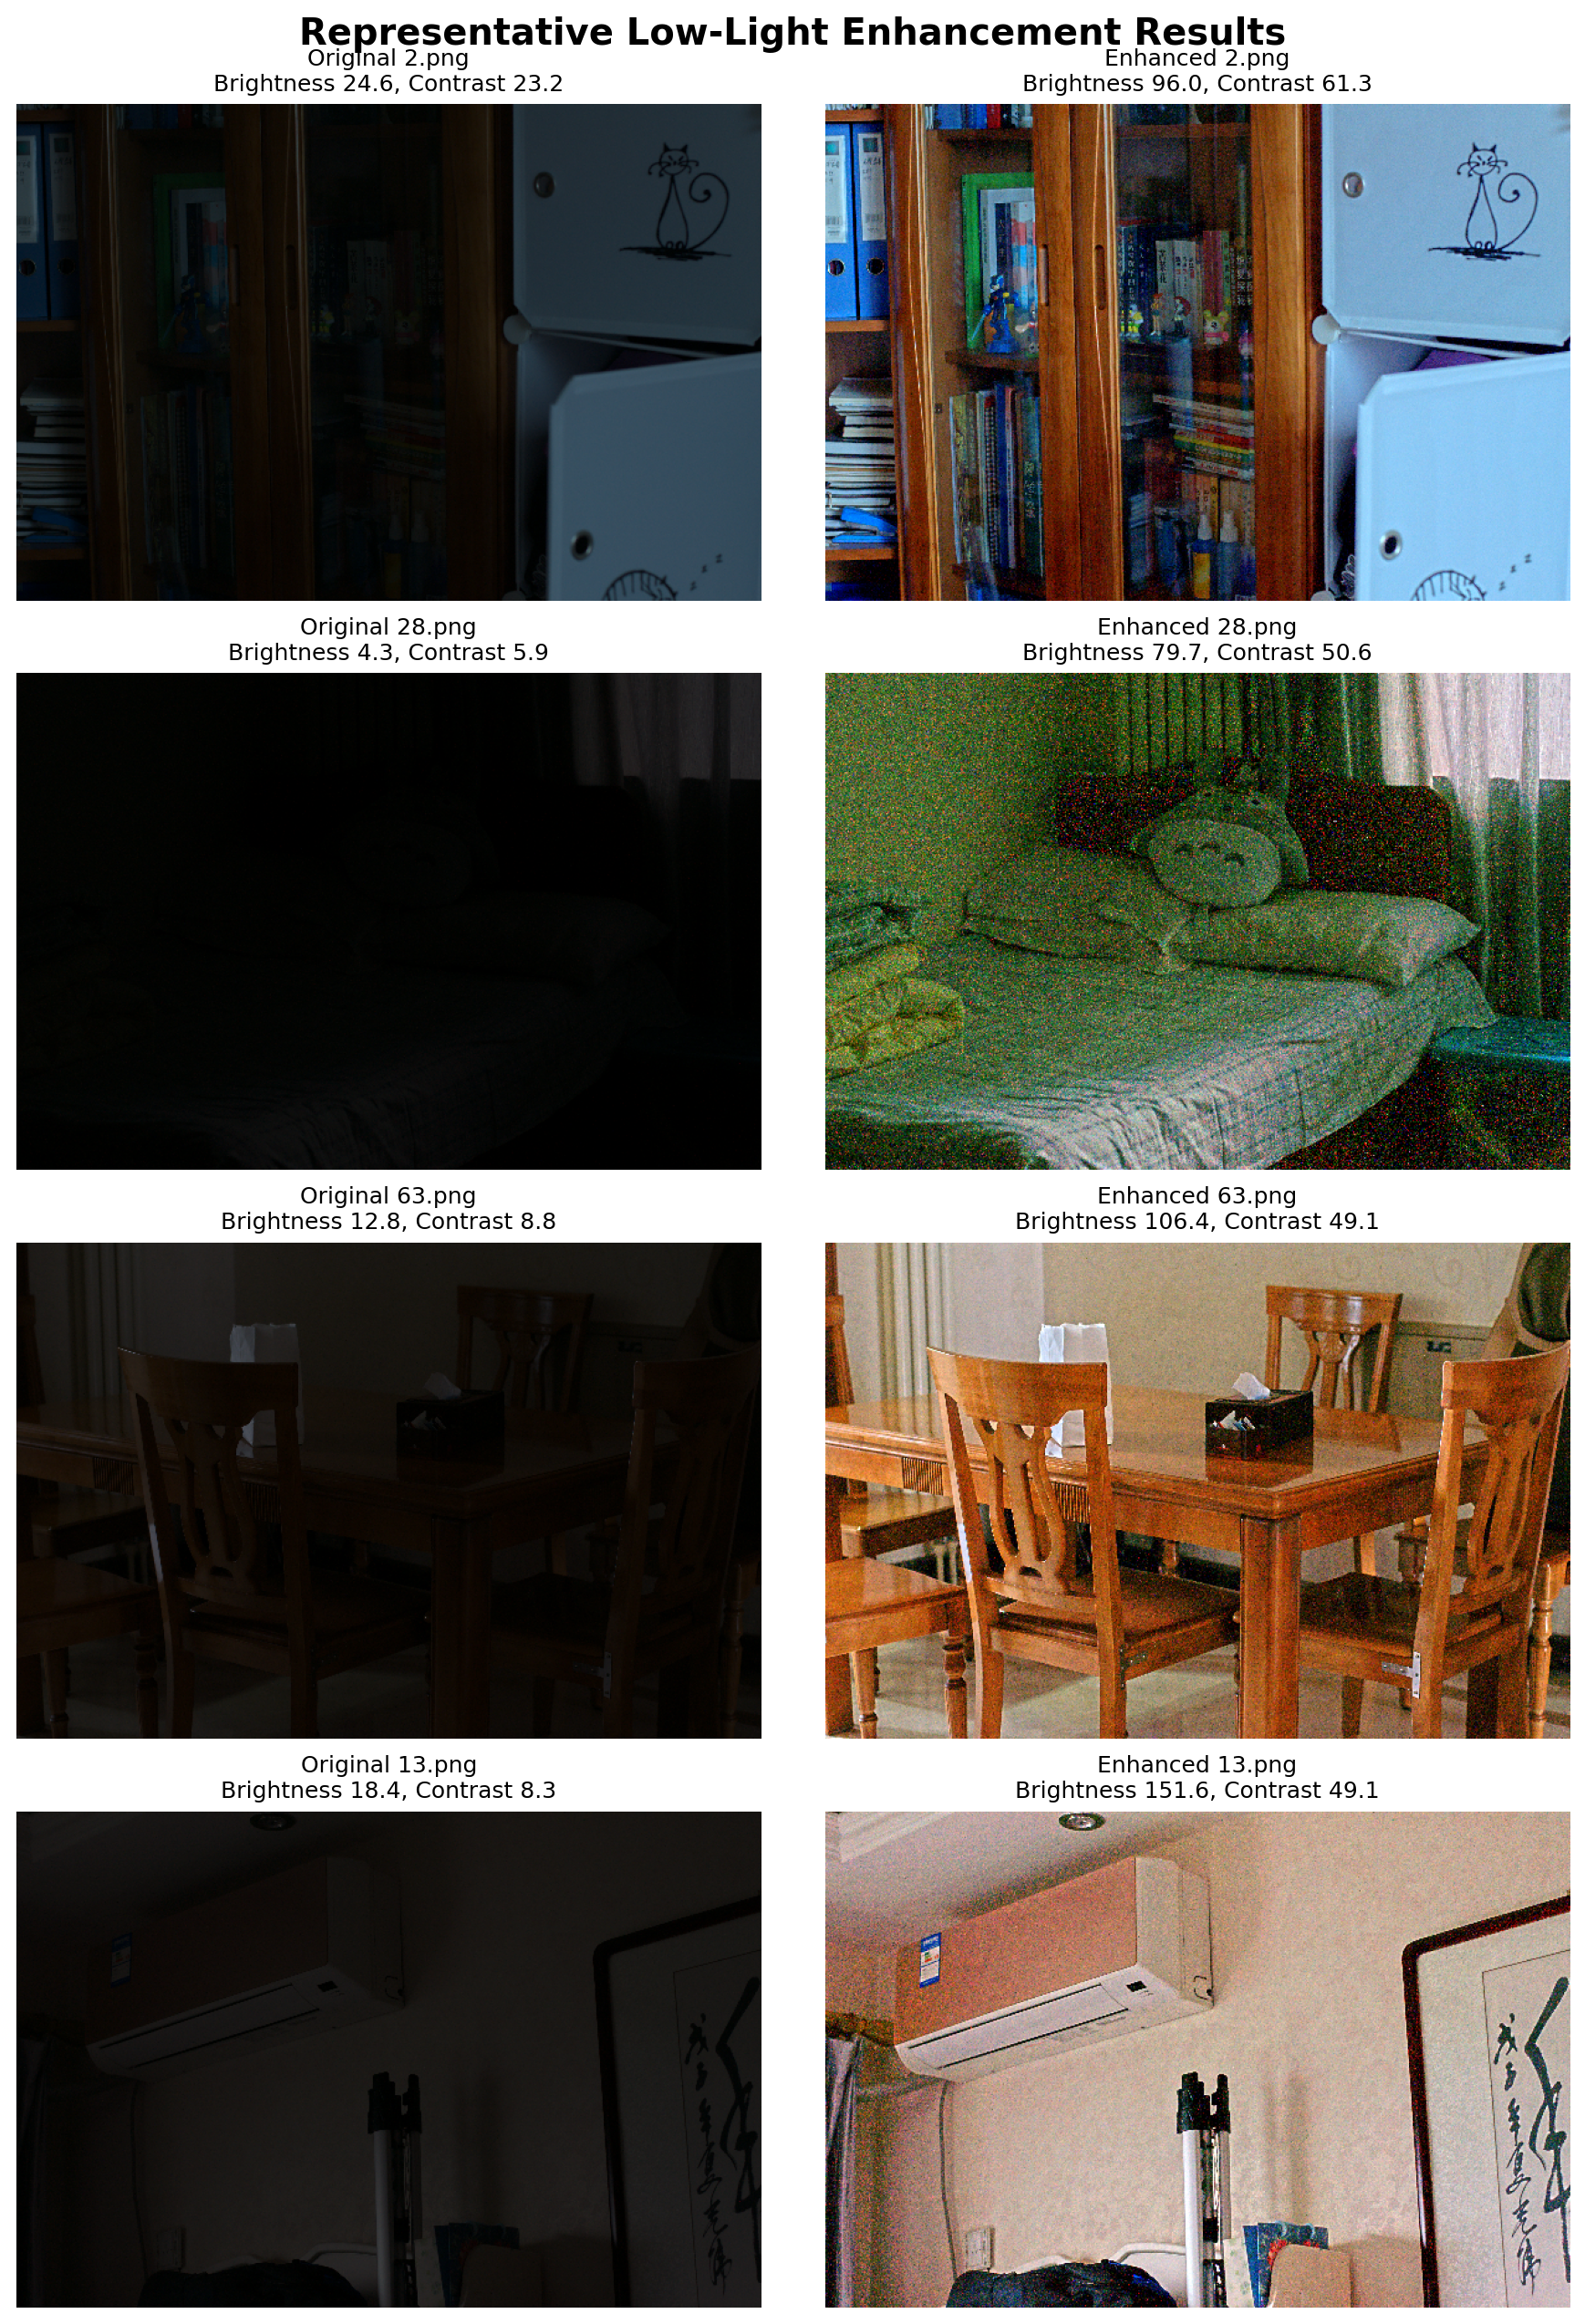
\includegraphics[width=0.95\textwidth]{sample_comparisons.png}
    \caption{Representative original and enhanced image comparisons from the dataset.}
    \label{fig:samples}
\end{figure*}

Qualitatively, the upgraded pipeline consistently increases scene visibility, expands local and global contrast, and assigns stronger gamma correction to darker regions. The decision to reconstruct from the original input rather than the denoised guide image also preserves a more natural level of detail.

\section{Quantitative Results}
Fig.~\ref{fig:metrics} summarizes average dataset-level quality metrics before and after enhancement. Fig.~\ref{fig:runtimegamma} shows how the auto-tuned gamma changes with input brightness and how runtime scales with image size.

\begin{figure}[t]
    \centering
    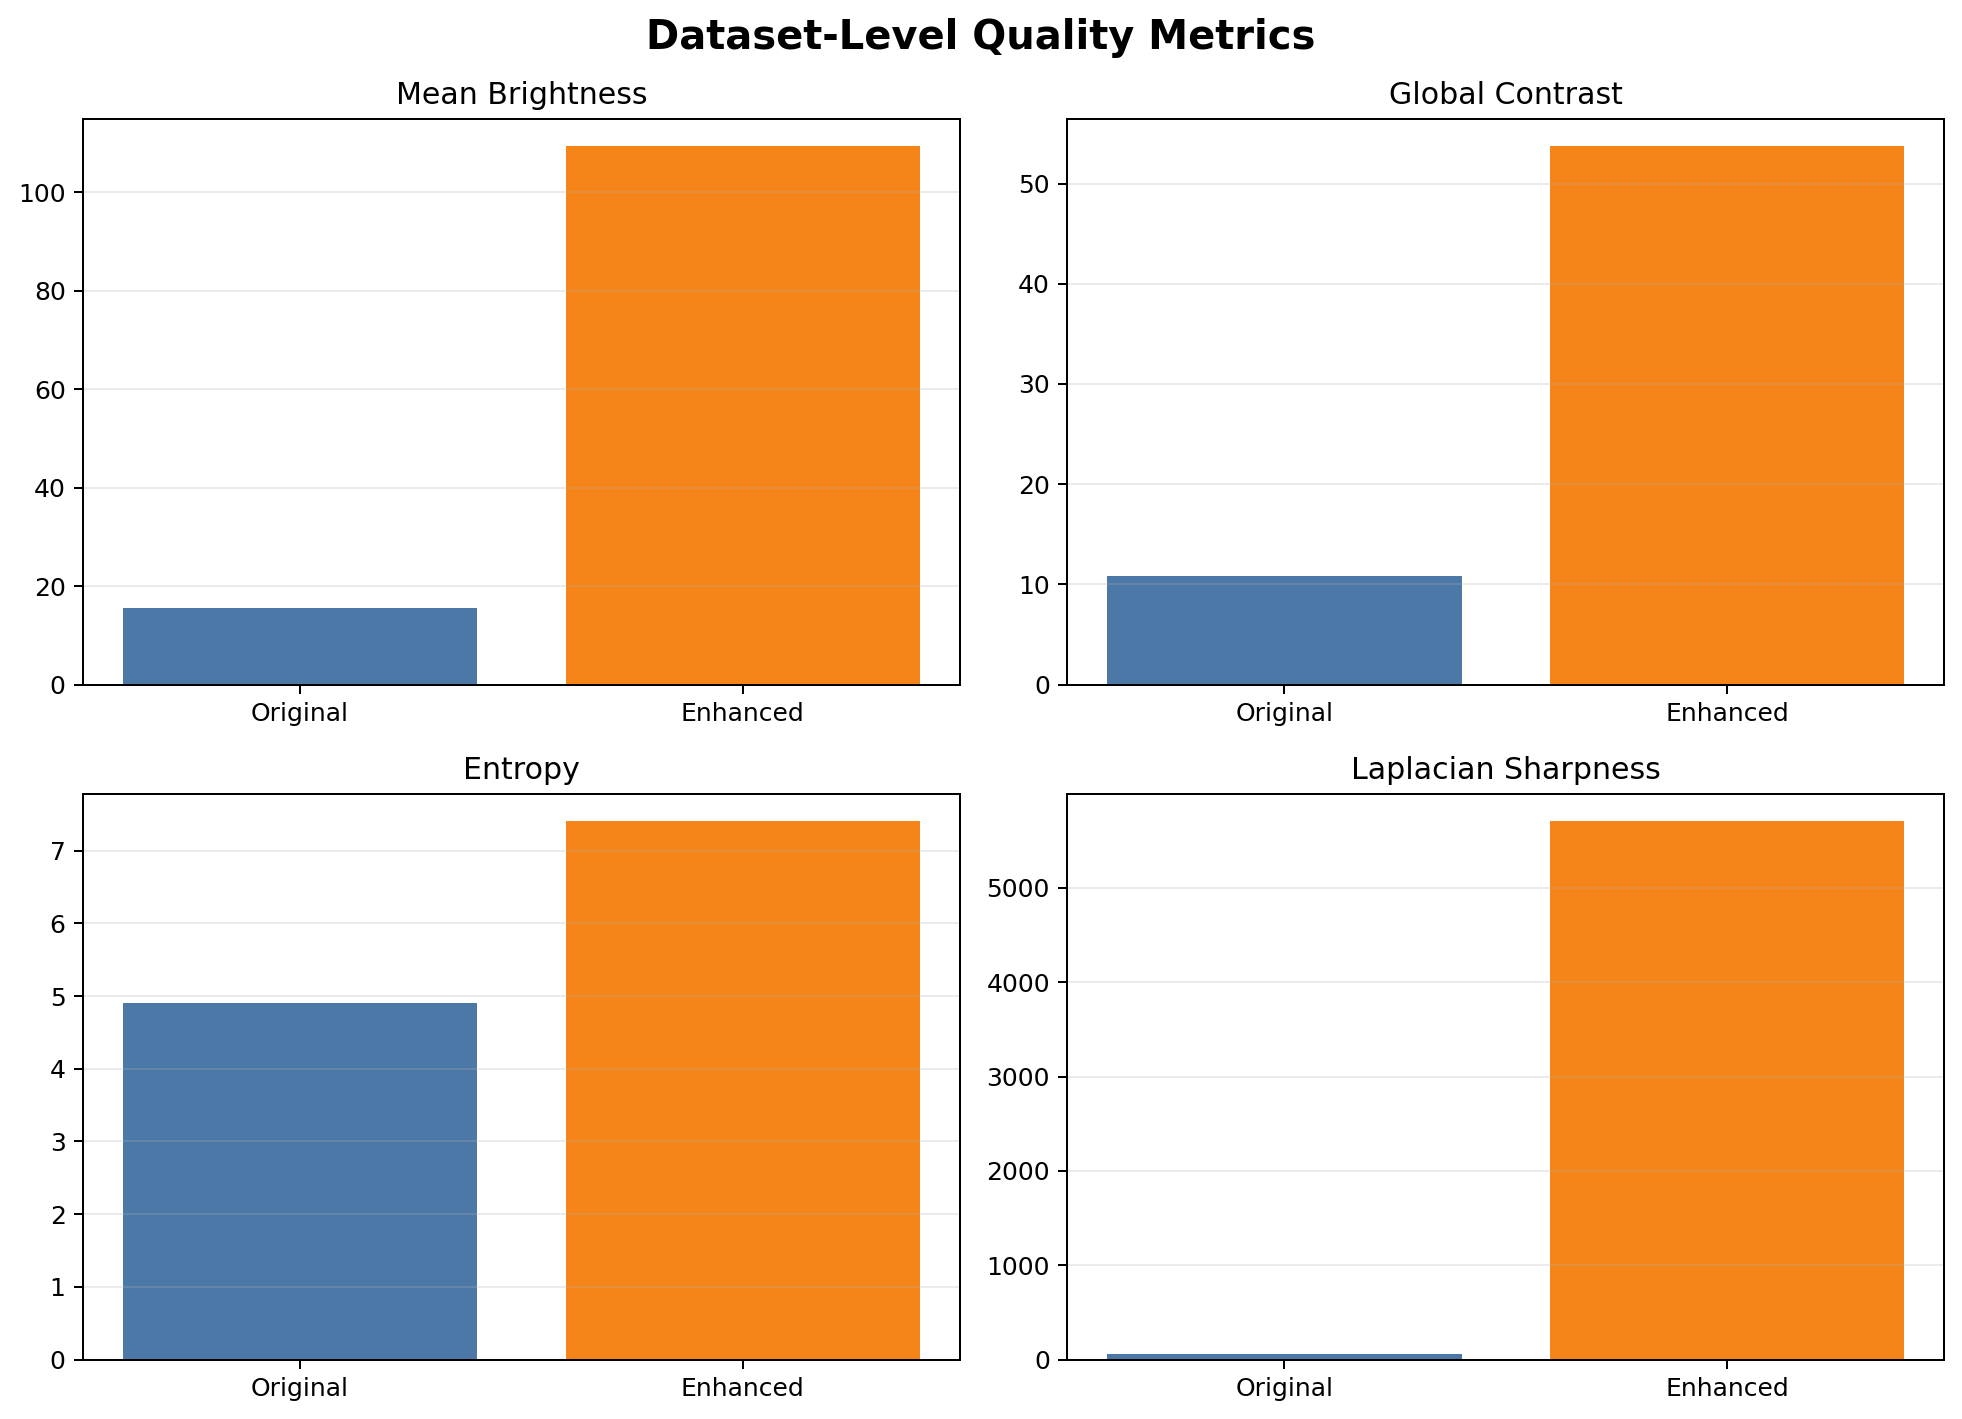
\includegraphics[width=\linewidth]{dataset_metrics.png}
    \caption{Dataset-level metric comparison for original and enhanced images.}
    \label{fig:metrics}
\end{figure}

\begin{figure}[t]
    \centering
    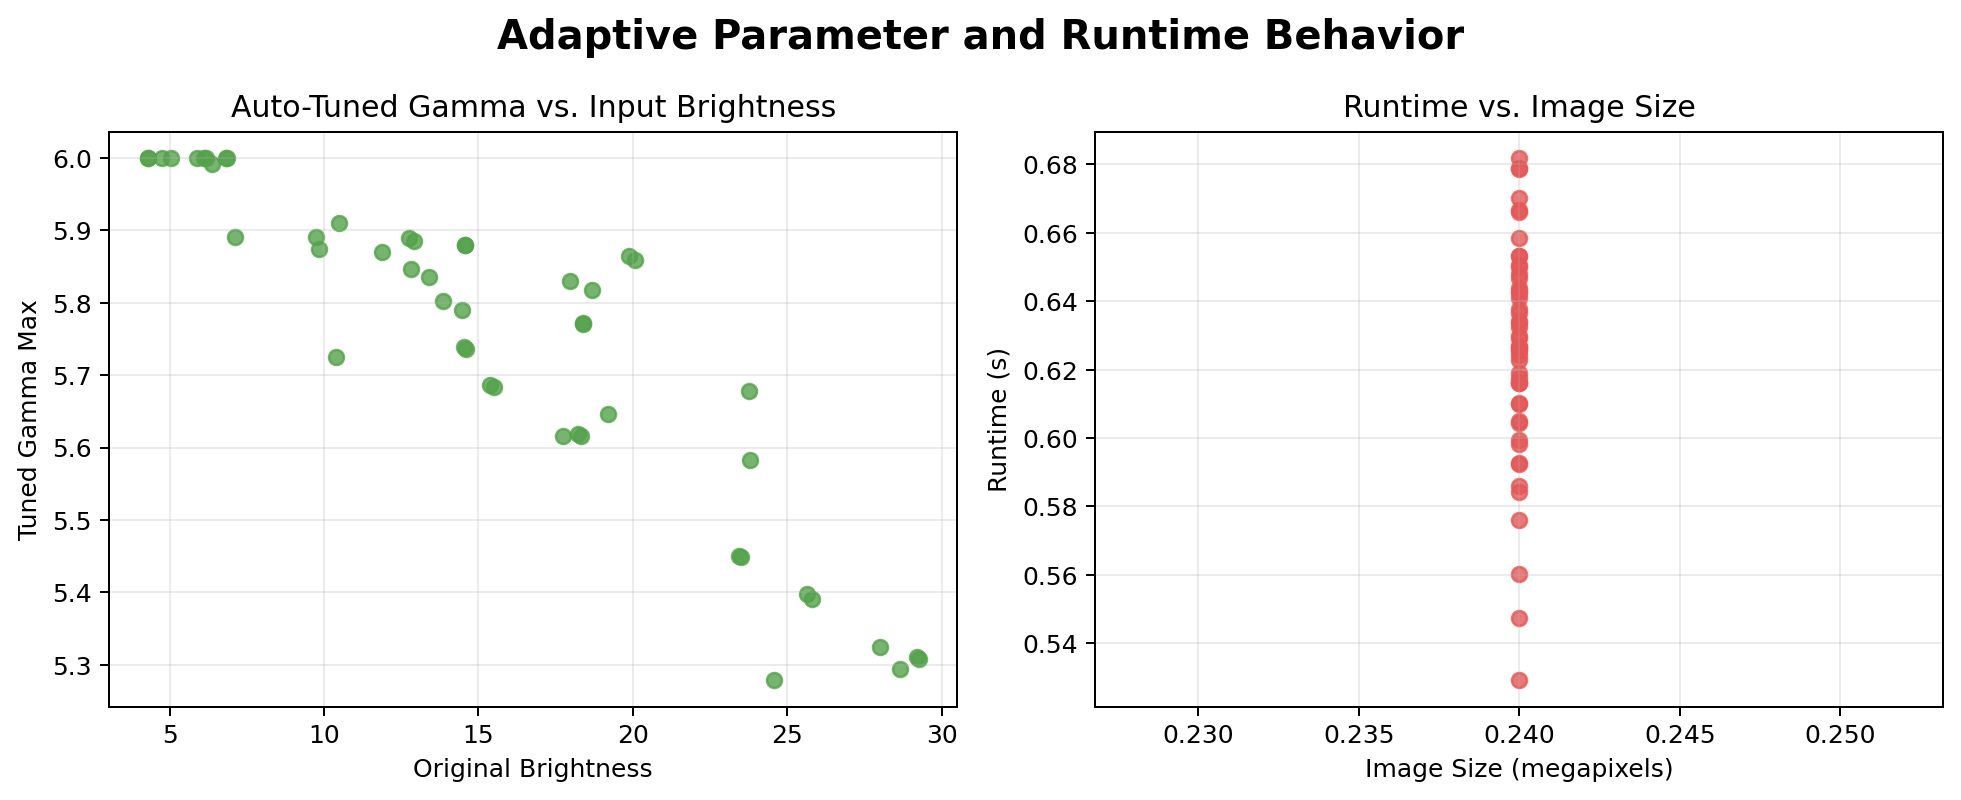
\includegraphics[width=\linewidth]{runtime_and_gamma.png}
    \caption{Adaptive gamma and runtime behavior across the dataset.}
    \label{fig:runtimegamma}
\end{figure}

Table~\ref{tab:aggregate} reports the average no-reference metrics over all 49 images.

\begin{table}[t]
    \caption{Average No-Reference Metrics Over the Dataset}
    \label{tab:aggregate}
    \centering
    \resizebox{\linewidth}{!}{%
    \begin{tabular}{lccc}
        \toprule
        Metric & Original Mean & Enhanced Mean & Delta \\
        \midrule
        Brightness & 15.468 & 109.333 & 93.865 \\
        Contrast & 10.791 & 53.721 & 42.930 \\
        Entropy & 4.904 & 7.405 & 2.501 \\
        Sharpness & 58.974 & 5706.727 & 5647.752 \\
        \bottomrule
    \end{tabular}
    }
\end{table}

Table~\ref{tab:samples} reports representative per-image results for four selected samples.

\begin{table}[t]
    \caption{Representative Sample Results}
    \label{tab:samples}
    \centering
    \resizebox{\linewidth}{!}{%
    \begin{tabular}{lccccc}
        \toprule
        Image & Bright. Gain & Contr. Gain & Entropy Gain & Gamma & Runtime \\
        \midrule
        2.png & 71.42 & 38.04 & 1.97 & 5.28 & 0.604 \\
        28.png & 75.42 & 44.69 & 3.65 & 6.00 & 0.529 \\
        63.png & 93.63 & 40.31 & 2.67 & 5.89 & 0.679 \\
        13.png & 133.27 & 40.83 & 2.28 & 5.77 & 0.638 \\
        \bottomrule
    \end{tabular}
    }
\end{table}

The average runtime was 0.625 s per image, with a minimum of 0.529 s and a maximum of 0.682 s on the evaluation set.

\section{Discussion}
The results indicate that the project enhancements improve both practicality and output quality.

\begin{enumerate}
\item The stronger denoising stage stabilizes light estimation in dark scenes.
\item Automatic gamma tuning removes the need to manually choose a single \texttt{gamma\_max} for every image.
\item Vectorization and reduced-resolution estimation improve efficiency without changing the overall algorithm design.
\item Reconstructing the final result from the original input avoids unnecessary smoothing and yields a more natural appearance.
\end{enumerate}

There are also several limitations. First, the metrics are no-reference and therefore do not directly measure fidelity against ground truth. Second, the strong increase in Laplacian variance partly reflects stronger edges and contrast, so it should be interpreted together with visual inspection. Third, the repository dataset is relatively small and contains similarly sized images, which limits runtime variability.

\section{Conclusion}
This project demonstrates a practical low-light enhancement system built on pixel-adaptive gamma correction and dehazing-inspired recovery. Three targeted implementation upgrades were added: stronger denoising, automatic parameter tuning, and faster processing. Evaluation on the repository dataset shows large gains in brightness, contrast, and entropy while maintaining visually stronger detail by recovering the final image from the original low-light input. The resulting codebase is more consistent, easier to analyze, and better suited for both demonstration and batch-processing workflows.

\section*{Acknowledgment}
The report is based on the repository implementation and references the original low-light enhancement paper of Jeon \textit{et al.}~\cite{jeon2023}.

\bibliographystyle{IEEEtran}
\bibliography{IEEE_Project_Report}

\end{document}
